\documentclass[tikz]{standalone}

%\usepackage{mathdots}
\usepackage[utf8]{inputenc}
\usepackage[upright]{fourier}
%\usepackage{tikz}
\usetikzlibrary{matrix,arrows,decorations.pathmorphing}

\newcommand\x{\times}

\begin{document}

% l' unite
\newcommand{\myunit}{1 cm}
\tikzset{
    node style sp/.style={draw,circle,minimum size=\myunit},
    node style ge/.style={circle,minimum size=\myunit},
    arrow style mul/.style={draw,sloped,midway,fill=white},
    arrow style plus/.style={midway,sloped,fill=white},
}


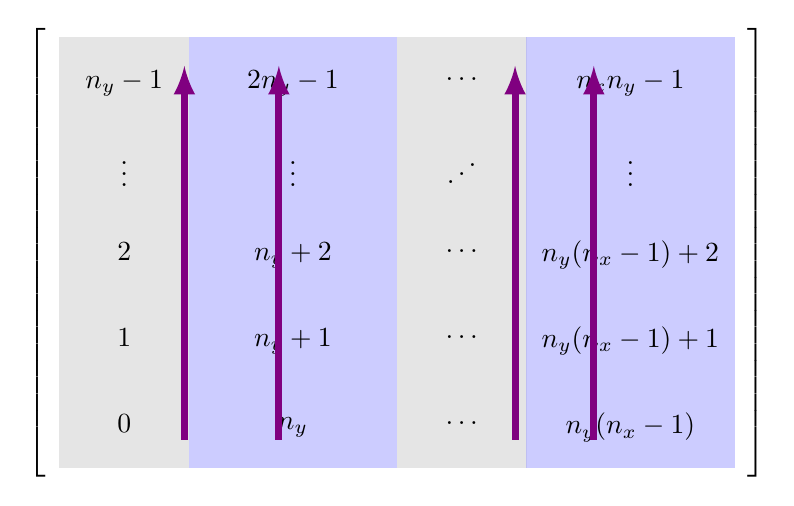
\begin{tikzpicture}[>=latex]
  %

  \matrix (A)
  [matrix of math nodes,
  nodes={rectangle, %draw, very thin,
    minimum size=1.2em, text depth=0.25ex,
    inner sep=0pt, outer sep=0pt,
    fill opacity=0.5, text opacity=1,
    anchor=center},
  column sep=-0.5\pgflinewidth,
  row sep=-0.5\pgflinewidth,
  %column 2/.append style = {nodes={fill=cyan!50}},
  %row 2/.append style = {nodes={fill=cyan!50}},
  every odd column/.style = {nodes={fill=gray!40}},
  every even column/.style = {nodes={fill=blue!40}},
  %row 2 column 2/.append style={nodes={fill=cyan}},
  row 1/.append style={nodes={minimum height=1.1cm}},
  row 2/.append style={nodes={minimum height=1.1cm}},
  row 3/.append style={nodes={minimum height=1.1cm}},
  row 4/.append style={nodes={minimum height=1.1cm}},
  row 5/.append style={nodes={minimum height=1.1cm}},
  column 1/.append style={nodes={minimum width=1.65cm}},
  column 2/.append style={nodes={minimum width=2.65cm}},
  column 3/.append style={nodes={minimum width=1.65cm}},
  column 4/.append style={nodes={minimum width=2.65cm}},
  left delimiter={[}, right delimiter={]}
  ]
{
  n_y-1  & 2 n_y-1 & \ldots                & n_x n_y-1  \\
  \vdots & \vdots  & \reflectbox{$\ddots$} & \vdots  \\
  2      &  n_y+2  & \ldots                & n_y(n_x-1)+2  \\
  1      &  n_y+1  & \ldots                & n_y(n_x-1)+1  \\
  0      &  n_y    & \ldots                & n_y(n_x-1)  \\
};

\node (P1) at (-2.7, -2.5) {};
\node (P2) at (-2.7,  2.5) {};
\draw[->,violet,line width=2.5] (P1) -- (P2);
\node (P3) at (-1.5, -2.5) {};
\node (P4) at (-1.5,  2.5) {};
\draw[->,violet,line width=2.5] (P3) -- (P4);
\node (P5) at ( 1.5, -2.5) {};
\node (P6) at ( 1.5,  2.5) {};
\draw[->,violet,line width=2.5] (P5) -- (P6);
\node (P7) at ( 2.5, -2.5) {};
\node (P8) at ( 2.5,  2.5) {};
\draw[->,violet,line width=2.5] (P7) -- (P8);

% \matrix (A) [matrix of math nodes,%
%              left delimiter  = {[},%
%              right delimiter = {]},
%              row 2/.append style = {nodes={fill=cyan!50}}] at (0,0)
% {%
%   n_x(n_y-1) & n_x(n_y-1)+1 & \ldots & n_x n_y-1  \\
%   \vdots & \vdots & \reflectbox{$\ddots$} & \vdots  \\
%   2n_x & 2n_x+1 & \ldots & 3n_x-1  \\
%   n_x & n_x+1 & \ldots & 2n_x-1  \\
%   0 & 1 & \ldots & n_x-1  \\
% };
%\node [draw,below=10pt] at (A.south)
%    { $A$ : \textcolor{red}{$n_x\times n_y$ row-major}};

\end{tikzpicture}
\end{document}
